\documentclass{article}
\usepackage{styles}

\title{Image Processing\\
    Lab 3}
\author{Kevin Gevers (s25595987) \\ Jeroen Overschie (s2995697)}
\date{\today}

\begin{document}

\maketitle

Note, that all used source code can be found attached next to this report's pdf file. Its structure should be self-explanatory; all requested functions are named accordingly and any extra functions are explained in the report. Note that (almost) every function has a corresponding test script, which is named just like its function, but with a suffix '\texttt{\_test}'. Where possible, we followed the terminology from the book \citep{gonzalez2008digital} for variable naming.

\section*{Exercise 1}
First some basic theory on the subject. We are given some grey scale image, $f$. We now denote the Laplacian pyramid of f using:
\[
    f_1 = f
\]
\[
\begin{aligned}
    f_j = \textsc{REDUCE}(f_{j-1}) & \text{  for $j=2,...J$}
\end{aligned}
\]

Please do denote the subtle differences between the lowercase $j$ and uppercase $J$. $J$ denotes the number of levels of the pyramid composition, e.g. when $J = 3$, the pyramid will consist out of 3 images: the original, a decomposition of the original, and a decomposition of the decomposition. Furthermore, we define $d_1,d_2,...d_{J-1}$ as the \textit{detail signals}, or \textit{residuals}:

\[
\begin{aligned}
    d_j = f_j - \textsc{EXPAND}(f_{j+1}) & \text{  for $j=1,2,...J-1$}
\end{aligned}
\]

Which are more simply said the decompositions scaled back to the dimensions of their previous form, to then get the difference between the two images using matrix subtraction. Because we are diffing the images here, our vector $d$ can only be of length $J-1$. Lastly, we define the \textsc{REDUCE} and \textsc{EXPAND} operators:

\[
    \textsc{REDUCE}(f) = \downarrow_2 (h_\sigma * f)
\]
\[
    \textsc{EXPAND}(f) = h_\sigma * (\uparrow_2 (f)),
\]

where $h_\sigma$ denotes \textit{Gaussian filtering}, which is a filter with a Gaussian response that can be used for performing a sort of image blur. The filter has the parameter $\sigma$, which is the standard deviation of the kernel. Furthermore, the operations denoted by the arrows, $\downarrow_2$ and $\uparrow_2$ denote \textbf{shrinking} and \textbf{zooming} an image by a factor $2$, respectively. In the spirit of maximum re-usability and efficiency, we reused some functions from Exercise 1 for this: the 'fundamental' functions \textsc{IPinterpolate} and \textsc{IPscaling\_transformation} to do the scaling work, and \textsc{IPdownsample} and \textsc{IPzoom} to apply them. These functions are thoroughly documented in the first report. In this lab, we use \textsc{IPdownsample} for our shrinking functionality ($\downarrow_2$) and \textsc{IPzoom} for zooming functionality ($\uparrow_2$).

\subsection*{(a)} In this first exercise, we were asked to implement a function \textsc{IPpyr\_decomp} that builds a Laplacian pyramid decomposition. For the parameters of this function, $f$ is the input image, $J$ the composition level and $\sigma$ the Gaussian filter kernel parameter. For our implementation, see \ding{118} Listing \ref{code:IPpyr_decomp}.

In our implementation, we use matlab \textit{Cell} types to store the pyramid and the detail signals, in variables $f$ and $d$, respectively. Note that the Matlab cell type indeed makes it possible to store matrices of variable lengths, though we do need the function \textsc{mat2cell} and \textsc{cell2mat} for storing/retrieving from the cell array. Like announced, we were allowed to use the function \textsc{imgaussfilt} to perform the Gaussian filtering process. We hand it a \textit{double} image (\textsc{im2double}) and the parameter $\sigma$. We perform both the Reducing and Expanding operations and store the residuals in $d$.

Now finally, we can store the result in a matrix $g$. We can compute the height for this result matrix using:


\[
    P = M \times (1+\frac{1}{2}+(\frac{1}{2})^2+...+(\frac{1}{2})^{J-1}),
\]

which we conveniently implemented using an element-wise squaring operation in Matlab, i.e. using \texttt{.\^} (see code line 25). Next come some basic geometry operations to stack the result images vertically over the space of $P$ and centering each image horizontally over the space of $M$. This done, we result with a result matrix $g$, which  is also saved to \texttt{IPpyr\_decomp-g\_J=3,sigma=1.0.mat}.
\subsection*{(b)} Next, we visualize the results, using again a \texttt{*\_test} script. See Figure ~\ref{fig:plant_original} for the original image and Figure~\ref{fig:plant_all_pyr-decomp} for its Laplacian pyramid decomposition using $J=3$ and $\sigma=1.0$.

\begin{figure}[h]
    \centering
    \includesvg[width=0.8\textwidth]{Assignment_3/output_plots/plant_original.svg}
    \caption{Original plant image for Exercise 1 without any filtering applied.}
    \label{fig:plant_original}
\end{figure}

\begin{figure}[H]
    \centering
    \includesvg[width=0.7\textwidth]{Assignment_3/output_plots/plant_all_pyr-decomp.svg}
    \caption{Laplacian pyramid decomposition of \ref{fig:plant_original} using $J=3$ and $\sigma=1.0$. Residuals $d$ are vertically stacked, with at the bottom the final decomposition, $f_{3}$.}
    \label{fig:plant_all_pyr-decomp}
\end{figure}

\subsection*{(c)} See \texttt{IPpyr\_decomp\_data-J=3,sigma=1.0.mat} for the result matrix data $g$.

\newpage
\section*{Exercise 2}
\subsection*{(a)}
For exercise 2 we are going to reconstruct the decomposed image from exercise 1. The exercise states \textit{"Let $f$ be a grey value image with Laplacian pyramid decomposition of $J$ levels given by detail signals $d_1, d_2, \ldots, d_{J - 1}$ and coarsest approximation $f_J$. As before you may assume that the image $f$ is a square image of size $M \times M$, where $M$ is a power of 2."} To reconstruct the image we need to use Formula \ref{eq:reconstruct}, which in turn needs Formula \ref{eq:expand}.

\begin{equation}\label{eq:reconstruct}
    f_{j}=\operatorname{EXPAND}\left(f_{j+1}\right)+d_j, \quad j=J-1, \ldots, 1
\end{equation}
\begin{equation}\label{eq:expand}
    \mathrm{EXPAND}(f)=h_{\sigma} *(\uparrow 2(f))
\end{equation}

Now we are tasked with writing a Matlab function \textit{IPpyr\_recon(g,J,sigma)} that implements the Laplacian pyramid reconstruction. Here $g$ is the decomposed image that was the result of exercise 1, $J$ is the number of decomposition levels, and \textit{sigma} is the standard deviation for the Gaussian filter. Our implementation can be seen in \ding{118} Listing \ref{code:IPpyr_recon}.

\subsection*{(b)}
Next we had to apply our function \textit{IPpyr\_recon(g,J,sigma)} to the result of exercise 1. We first load the .mat file that was saved in Exercise 1, extract the coarsest level image, $f_J$ and then apply our reconstruction function \textit{IPpyr\_recon} to it. See \ding{118} Listing \ref{code:IPpyr_recon_test}, for the final testing code.

Figure \ref{fig:2b} shows the input image and the reconstructed image side by side. Here we used $J = 3$ and $sigma = 1.0$ as stated in the assignment.

\begin{figure}[h]
    \centering
    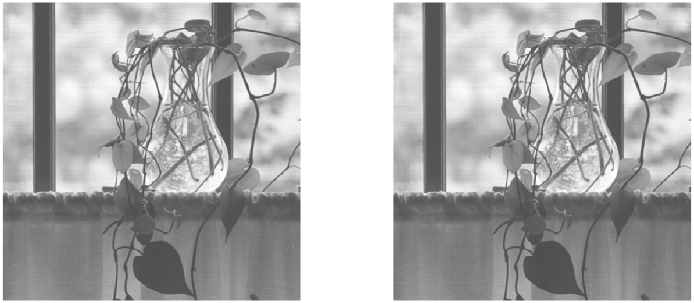
\includegraphics[width=\textwidth]{Assignment_3/output_plots/IPpyr_recon_test_partial.png}
    \caption{(Left) Input image. (Right) Reconstruction of the image after having decomposed it.}
    \label{fig:2b}
\end{figure}

\subsection*{(c)}
The next step is to calculate the mean absolute error between the reconstructed image and the input image. For this we need to use Formula \ref{eq:meanabserror} and we need to make sure both images are of the same type (which is \textit{double} for us).

\begin{equation}\label{eq:meanabserror}
    \operatorname{error}(f, g)=\frac{1}{M \times N} \sum_{i=1}^{M} \sum_{j=1}^{N}|f(i, j)-g(i, j)|
\end{equation}

We also need to compute the difference image between the input and reconstructed images. This is done by taking the mean absolute value of each pixel value using both images. The result is presented in Figure \ref{fig:recon_all}.

$^*$Note: We used the input image converted to the type \textit{double} and the reconstructed image which was already of the type \textit{double}. So we did not convert our reconstructed image to \textit{uint8} as stated in the assignment, seeing as that gave very weird and incorrect results.

\subsection*{(d)}

\begin{figure}[h]
    \centering
    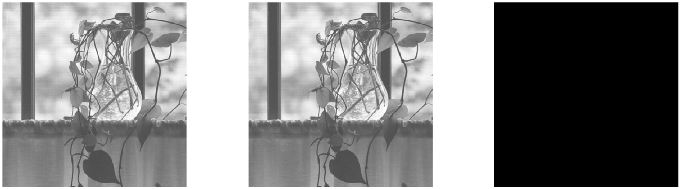
\includegraphics[width=\textwidth]{Assignment_3/output_plots/IPpyr_recon_test.png}
    \caption{(Left) Input image. (Middle) Reconstruction of the image after having decomposed it. (Right) Difference image between the input image and reconstructed image.}
    \label{fig:recon_all}
\end{figure}
The last part of the assignment is to put the input image, the reconstructed image, and the difference image together in a single figure and save it. We did this as can be seen in \ding{118} Listing \ref{code:IPpyr_recon_test} and in Figure \ref{fig:recon_all}. The mean absolute error between the two images as implemented in (c) gives us the error $0.0252$, which seems very reasonable when we look at the difference image in Figure \ref{fig:recon_all}.

\bibliographystyle{plain}
\typeout{}
\bibliography{Assignment_3}

\newpage
\appendix
\section{Code}
\subsection{Exercise 1}
\lstinputlisting[caption={\textsc{IPpyr\_decomp} function: Laplacian pyramid decomposition.}, label={code:IPpyr_decomp}]{Assignment_3/IPpyr_decomp.m}
\subsection{Exercise 2}
\subsubsection{Exercise 2 (a)}
\lstinputlisting[caption={\textsc{IPpyr\_recon} function: Laplacian pyramid reconstruction.}, label={code:IPpyr_recon}]{Assignment_3/IPpyr_recon.m}
\subsubsection{Exercise 2 (b-d)}
\lstinputlisting[caption={\textsc{IPpyr\_recon\_test} test script: executing the various task from exercise 2b-d.}, label={code:IPpyr_recon_test}]{Assignment_3/IPpyr_recon_test.m}
\end{document}
